\chapter{Background Estimation}

\section{Introduction}

The Standard Model backgrounds to the search are estimated in 16 bins of ($\HT$,
$\MET$). The $\HT$ bins are $400-500\unit{GeV}$, $500-600\unit{GeV}$,
$600-700\unit{GeV}$ and $700\unit{GeV}+$ and the $\MET$ bins are
$50-100\unit{GeV}$, $100-150\unit{GeV}$, $150-200\unit{GeV}$ and
$200\unit{GeV}+$. Only the ($\HT>700\unit{GeV}$, $\MET>200\unit{GeV}$) bin is
significant in terms of setting a limit on the GMSB cross-section. The other
bins are used only to give confidence in the background estimation procedure. \\

The main background comes from QCD processes. These events have only fake $\MET$
due to detector imperfections. The size of the QCD background is estimated using 
a control sample from the data. \\

The electroweak background is small in comparison to the QCD background.
Electroweak processes can contribute real $\MET$ through the production of
neutrinos that are not detected. The size of the electroweak background is 
estimated using MC.

\section{QCD Background}
\label{sec:QCD_Background}

The largest background comes from QCD processes. There are three different 
components to the QCD background:

\begin{itemize}
\item {\bf Fakes from jets ($\pi^{0}\rightarrow\gamma\gamma$):} $\pi^{0}$s are
one of the main constituents of jets. The two photons from a high energy 
$\pi^{0}$ can easily be mistaken for a single photon. Most $\pi^{0}$s will be 
non-isolated due to the surronding jet. However there is a distribution of 
isolation and given the large cross section of QCD, some of these events will 
end up in the isolated tail.
\item {\bf Prompt $\gamma$+jet:} In these events the photon comes directly from
the parton hard scattering. The other jet can come from gluon radiation or
jet fragmentation. These events contain prompt photons which tend to be isolated
and have good shower shape. The $\pT$ of the photons is distributed around half
the $\HT$ of the event.
\item {\bf QCD jets with ISR/FSR:} A QCD jets event where an initial state quark
or final state quark radiates a photon. These events also contain prompt photons
which tend to be isolated and have good shower shape. The cross section of this 
process falls with the $\pT$ of the photon. 
\end{itemize}

QCD events are balanced in the transverse plane. All three sources of QCD 
background have only fake $\MET$. Fake $\MET$ can come from the HCAL resolution, 
severe mismeasurements such as dead ECAL Trigger Towers, poor HCAL response or 
from fluctuations inherent in the hadronic showering process. \\

ECAL Trigger Towers are groups of ECAL crystals used for triggering and readout.
Some of the trigger towers are dead (i.e. there is no data coming from them).
Any object going down a dead trigger tower will be missed causing fake $\MET$.
There are also individual dead cells. Figure \ref{fig:Dead_ECAL_TTs} shows a map 
of the ECAL barrel with the dead regions marked. \\

\begin{figure}
\begin{center}
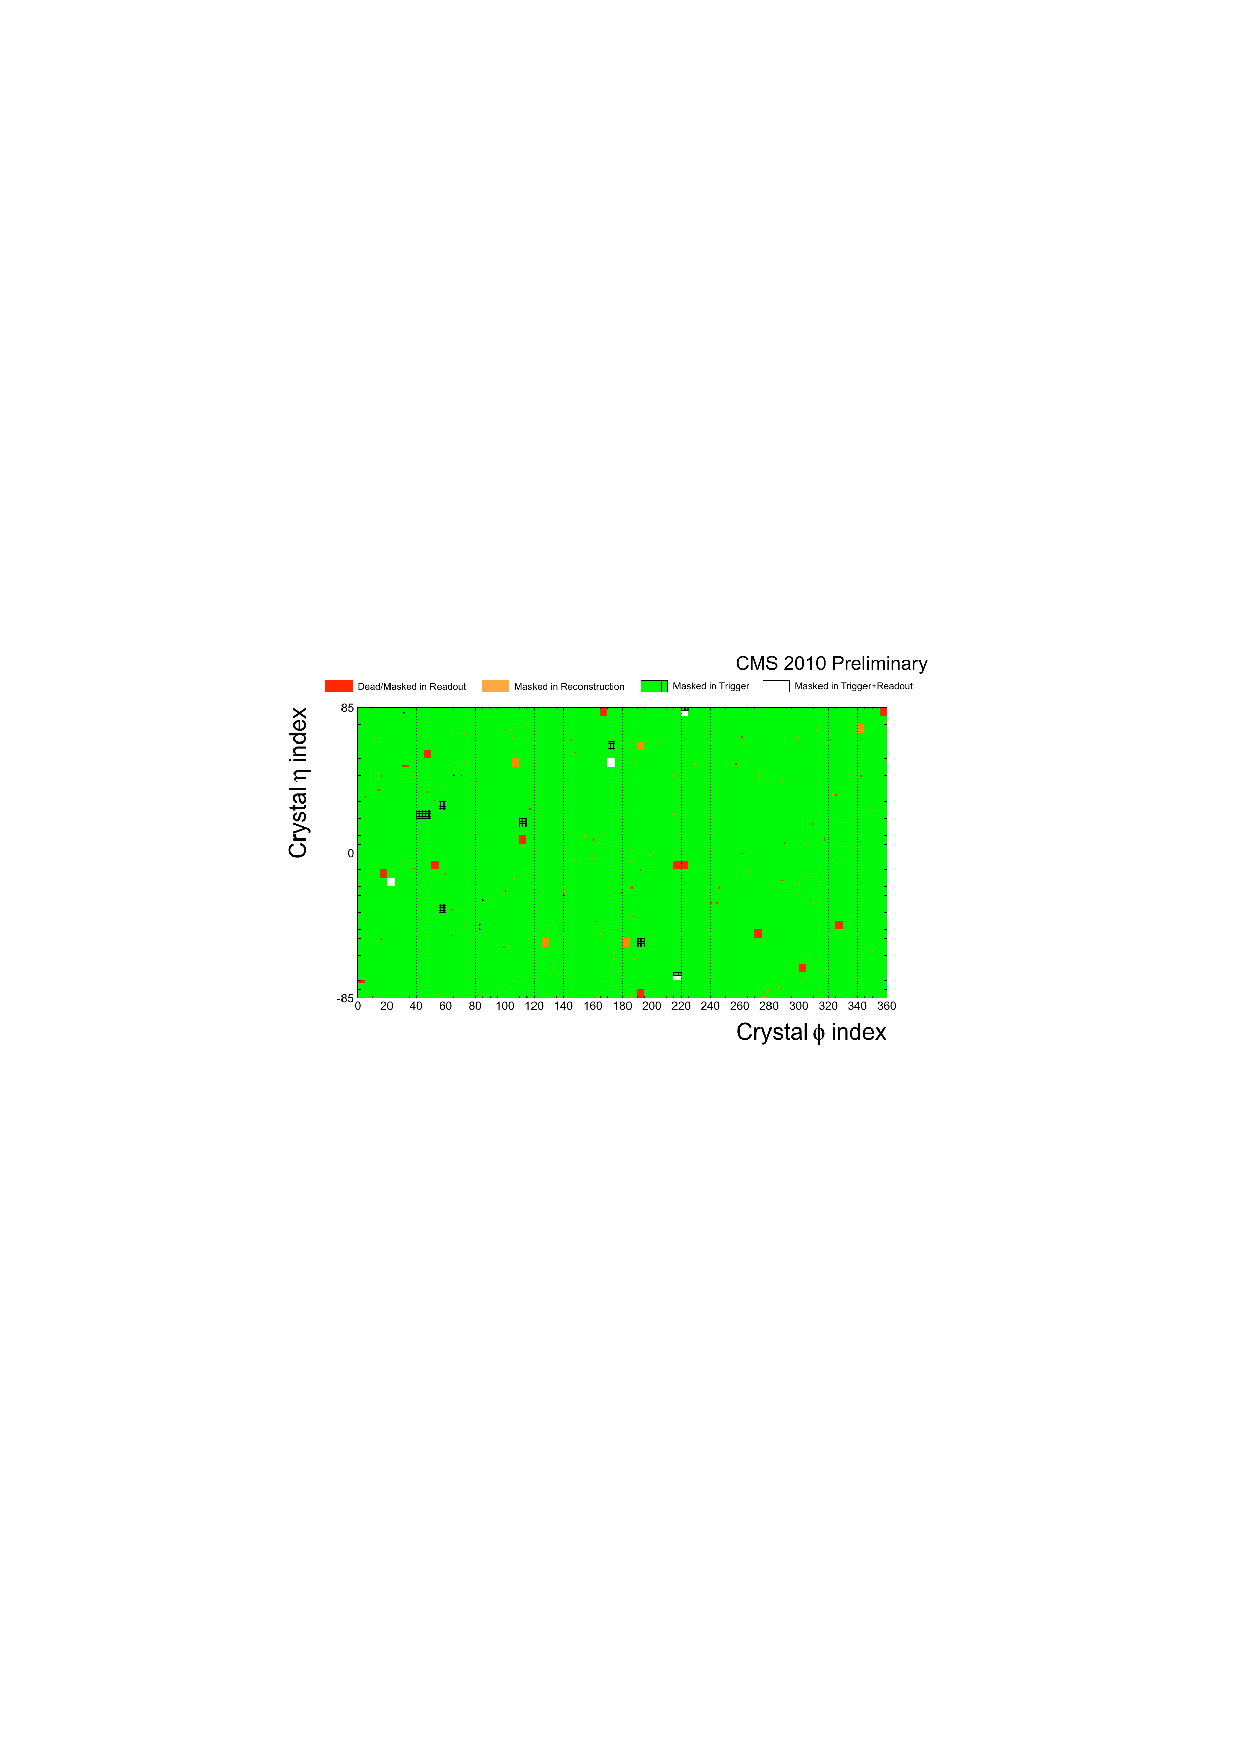
\includegraphics[width=\textwidth]{Ecal_Dead_TTs.pdf}
\end{center}
\caption{A map of the ECAL barrel showing the dead regions. Reproduced from 
\cite{spikes}.}
\label{fig:Dead_ECAL_TTs}
\end{figure}

There are also resolution effects which can cause fake

Poor HCAL response is another cause of large fake $\MET$. Sometimes a jet is
reconstructed with a much lower $\pT$ than it actually has. Such mismeasurements
are extremely pathelogical and not at all well understood. These are not
correlated with any specific region of the detector. \\

The core resolution is approximately Gaussian in x and y components of $\MET$ 
while the severe mismeasurements contribute a non-Gaussian tail to the $\MET$ 
distribution. Both components scale up with $\HT$. The core resolution scales as
$\sim\sqrt{\HT}$ while the tails increase because higher $\HT$ events contain 
higher $\pT$ objects which give larger $\MET$ when missed. \\

Any background estimation method needs to be able to estimate these detector 
effects. If the Monte Carlo were to be used we would be relying on its ability 
to correctly model all the causes of fake $\MET$. Not just the core resolution 
but also the $\MET$ tail with severe mismeasurements. Using a control sample 
from data gives a perfect simulation of the CMS detector. The problem is reduced
to finding a control sample with the same kinematic properties as the selected 
sample rather than trying to simulate the most extreme elements of detector
response. \\

A control sample is defined to contain events which pass all the selection 
criteria except for the isolation. This control sample is used to estimate the
$\MET$ shape of the QCD background in each $\HT$ bin. The absolute number of
events is obtained by normalising the $\MET$ distribution to the number of
events with $\MET < 50 \unit{GeV}$. \\

The assumption in this method is that the control sample has the same $\MET$
distribution as the selected sample in each $\HT$ bin. The control sample is
very similar to the selected sample. It has the same objects with the same
kinematic cuts. All events contain at least one photon with good shower shape.
The only difference is that in the control sample the photon is non-isolated
while in the selected sample it happens to be isolated. Although they contain
the three sources of QCD background in different proportions, in both cases the 
source of $\MET$ is the same: detector effects. So we can expect them to have 
the same $\MET$ distributions. \\

The background estimation is shown to work in Monte Carlo and in data using a 
sideband region. Figure \ref{fig:Regions} shows the regions used for the
background estimation. The (non-isolated) control sample is used to estimate the 
background in the (isolated) selected sample. The sideband region is used to
check that the background estimation works i.e. the non-isolated and isolated 
samples have the same $\MET$ distribution. \\

\begin{figure}
\begin{center}
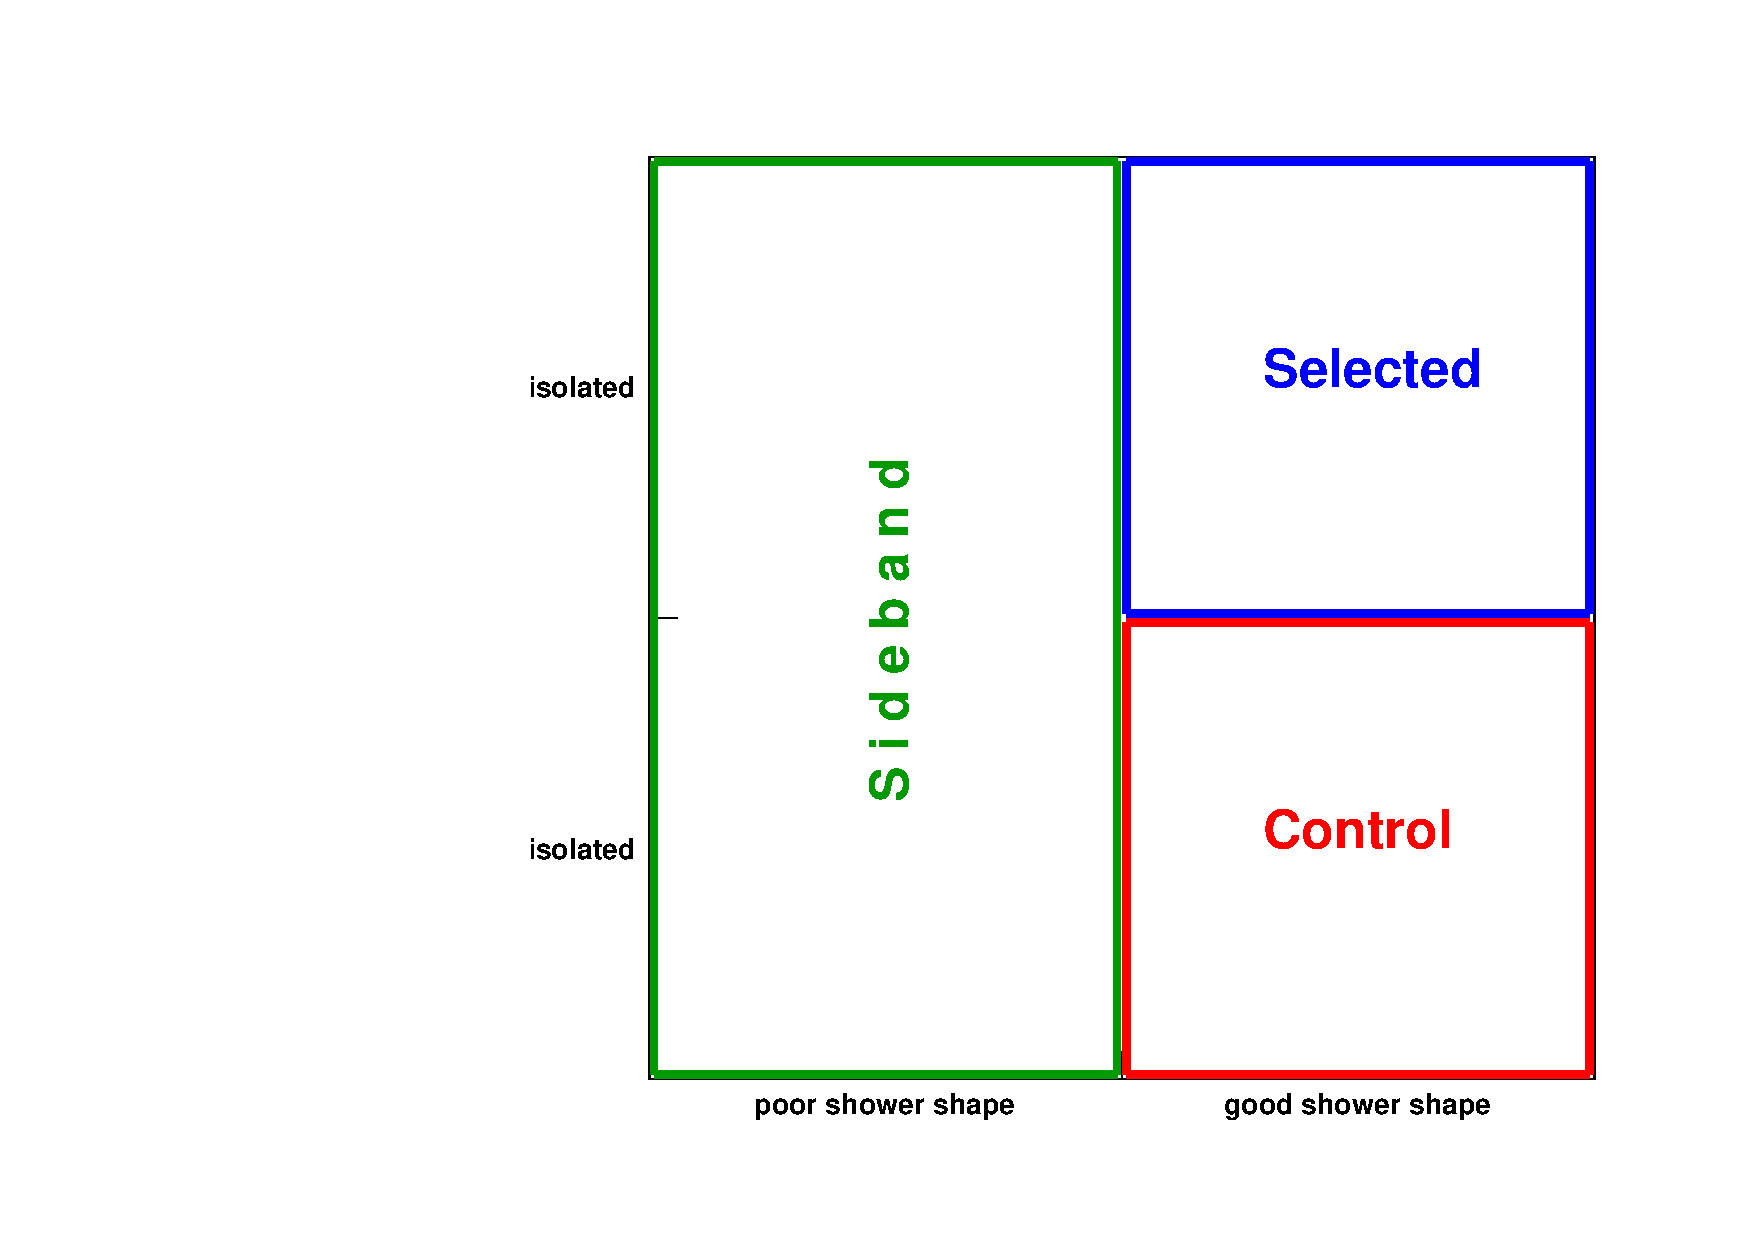
\includegraphics[width=0.8\textwidth]{Regions.pdf}
\end{center}
\caption{A graphic showing the layout of the regions used for the QCD background
estimation. The control sample is used to estimate the $\MET$ distribution in
the selected sample. The sideband region is used to check that the background
estimation works.}
\label{fig:Regions}
\end{figure}

To assess how well the background estimation technique works, the $\MET$
distribution of the selected events is compared to the prediction of the 
$\MET$ distribution using the control sample. This is done using the MC and the
sideband region to give two independent checks each with different qualities.
The check of the background estimation using the MC shows how well the technique
works in principle. It has the advantage that it is probing a kinematically
identical regoin to the data, but the disadvantage that the MC does not
accurately reproduce the $\MET$ distribution in data. The check of the 
background estimation technique using the sideband region in data uses a 
kinematically similar, but not idential region. It has the advantage that being 
from data it reliably reproduces the detector idosyncracies which cause the fake 
$\MET$. \\

Figure \ref{fig:Bkgd_Est_MC} shows the $\MET$ distribution in the MC for the 
selected events compared to the prediction of the $\MET$ distribution using the 
control sample. The data are split bins of $\HT$: $400-500\unit{GeV}$, 
$500-600\unit{GeV}$, $600-700\unit{GeV}$ and $700\unit{GeV}+$. The ratio of the 
number of events in the selected sample to the number of events predicted using 
the control sample. A straight line is fitted to the ratio plot to give a 
quantatative measure of the performance of the background estimation. The 
important number to compare is the number of events in the search bin
($\HT>700\unit{GeV}$, $\MET>200\unit{GeV}$), which is predicted to be 
$0.17\pm0.04$ using the control sample in the MC. The true value in the MC is 
$0.24\pm0.06$. \\

\begin{figure}
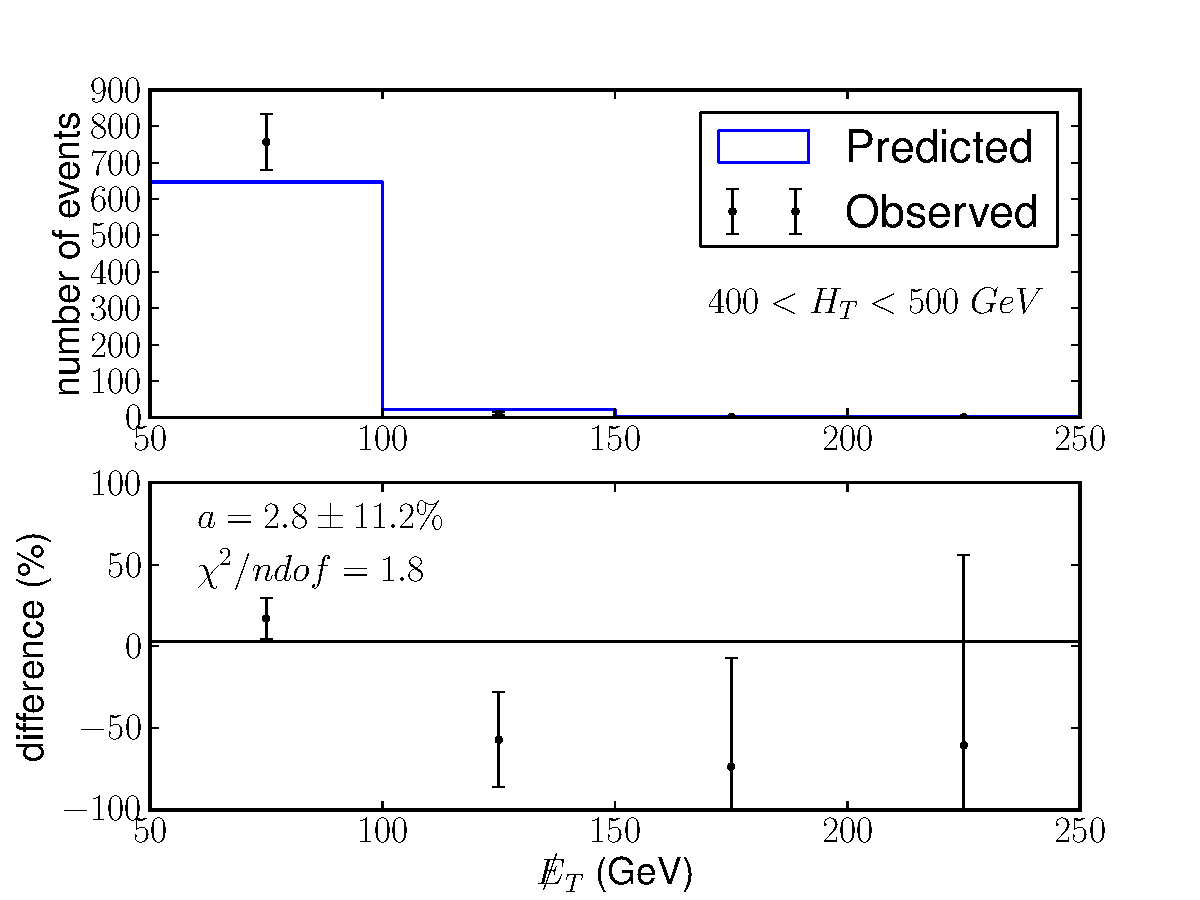
\includegraphics[width=0.5\textwidth]{MC_Bkgd_Est_1.pdf}
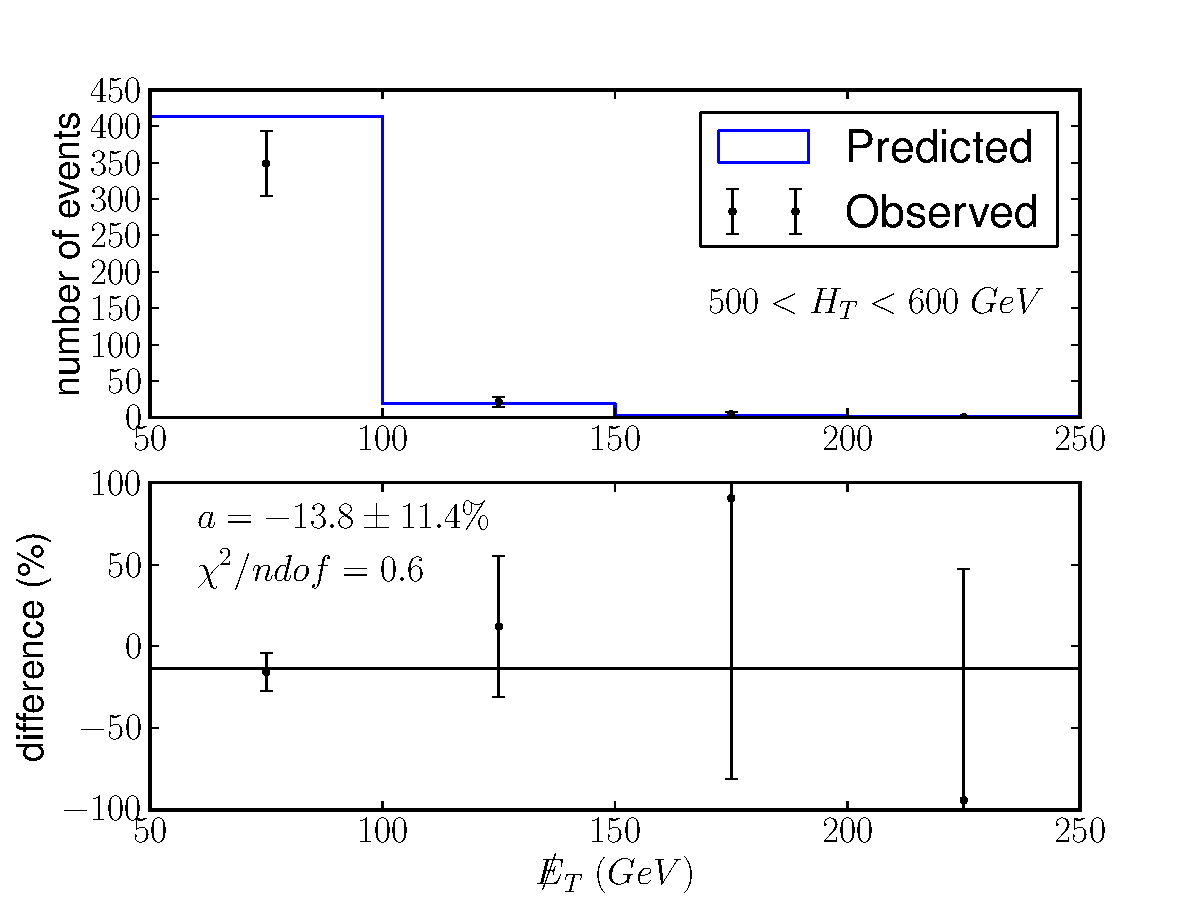
\includegraphics[width=0.5\textwidth]{MC_Bkgd_Est_2.pdf}\\
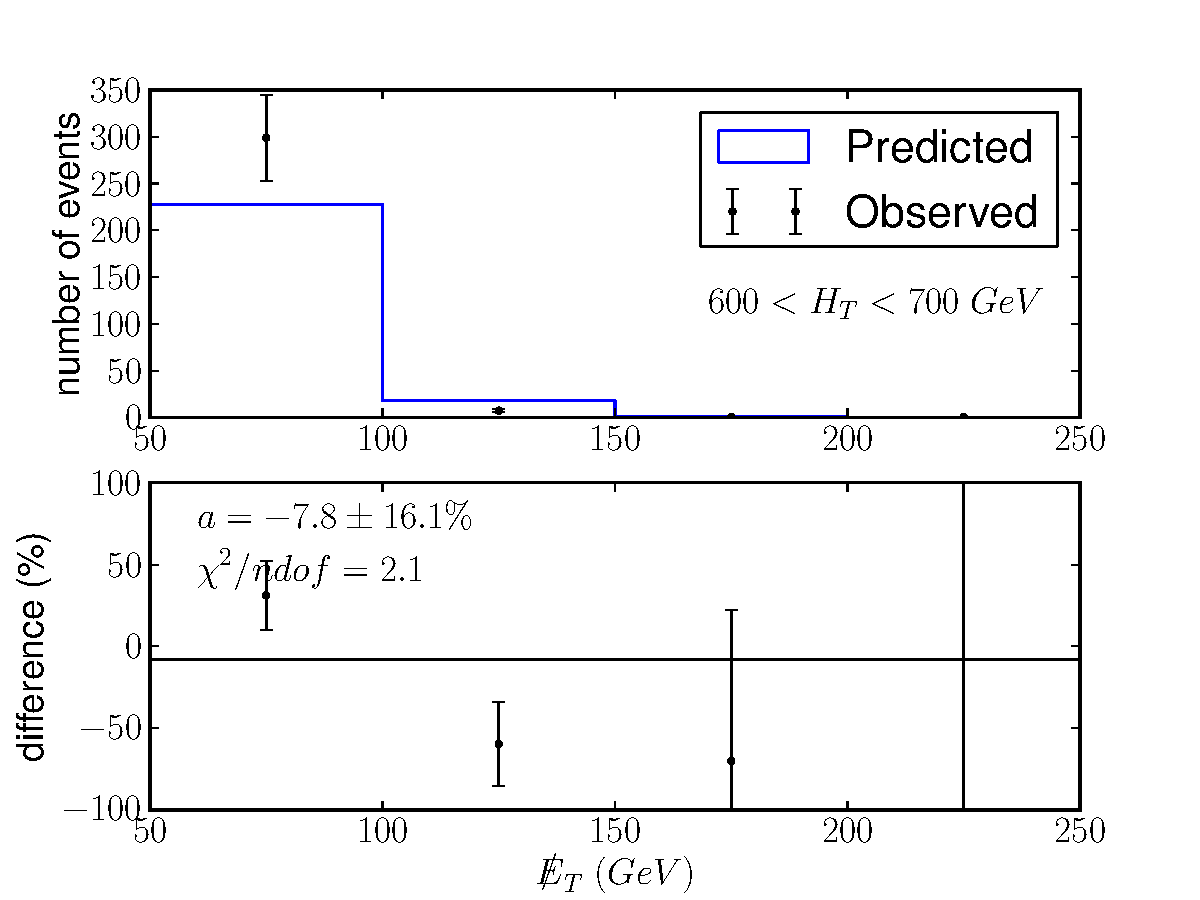
\includegraphics[width=0.5\textwidth]{MC_Bkgd_Est_3.pdf}
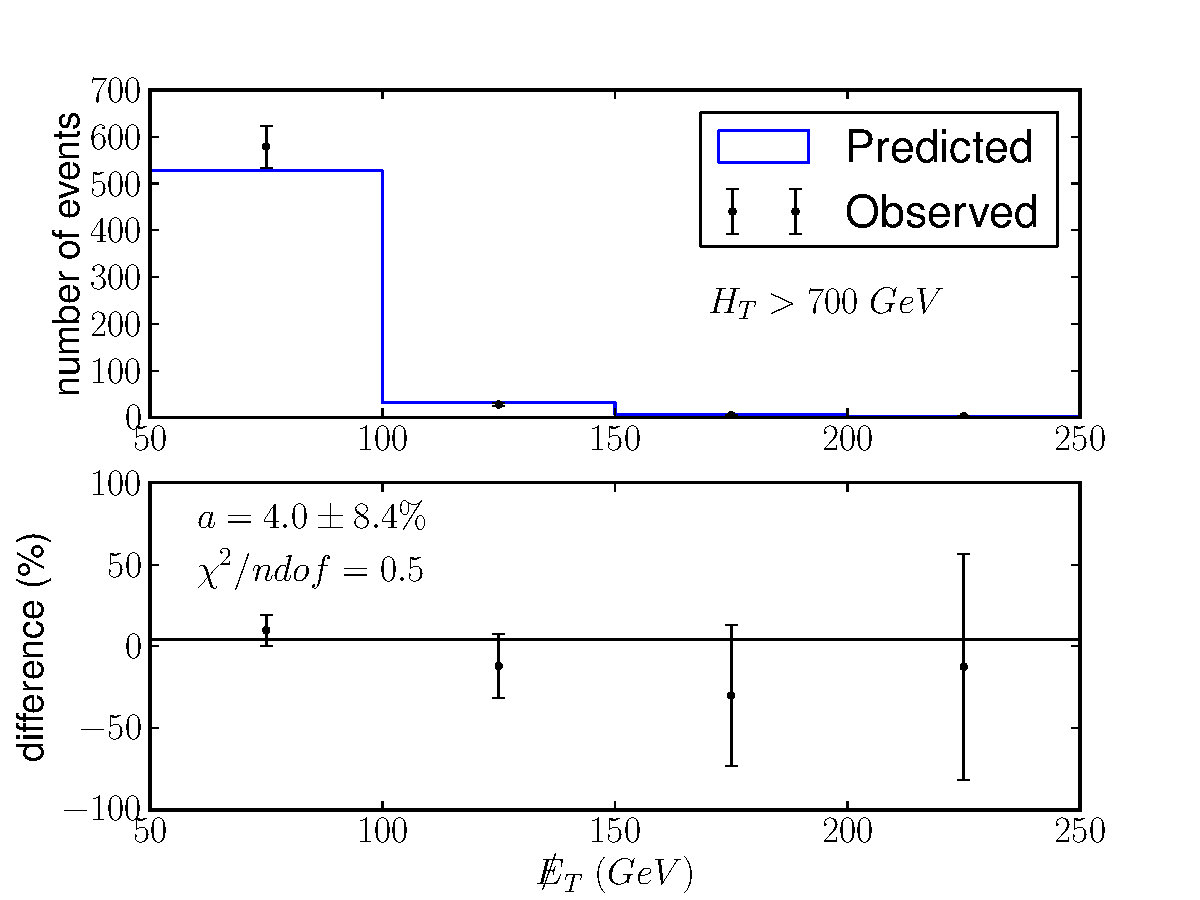
\includegraphics[width=0.5\textwidth]{MC_Bkgd_Est_4.pdf}\\
\caption{The estimation of the $\MET$ distribution of the background using the
control sample in the MC compared to the true $\MET$ distribution of the 
background according to the MC in bins of $\HT$. The percentage difference 
between the estimated and observed number of events is plotted and a flat line 
is fitted.}
\label{fig:Bkgd_Est_MC}
\end{figure}

Figure \ref{fig:Bkgd_Est_Sideband} shows the predicted and observed $\MET$ 
distribution in the sideband region. The number of events in the search bin for
the sideband region is predicted to be $0.09\pm0.04$ compared to an observation of
0. The prediction is consistent with the observed number of events. \\

\begin{figure}
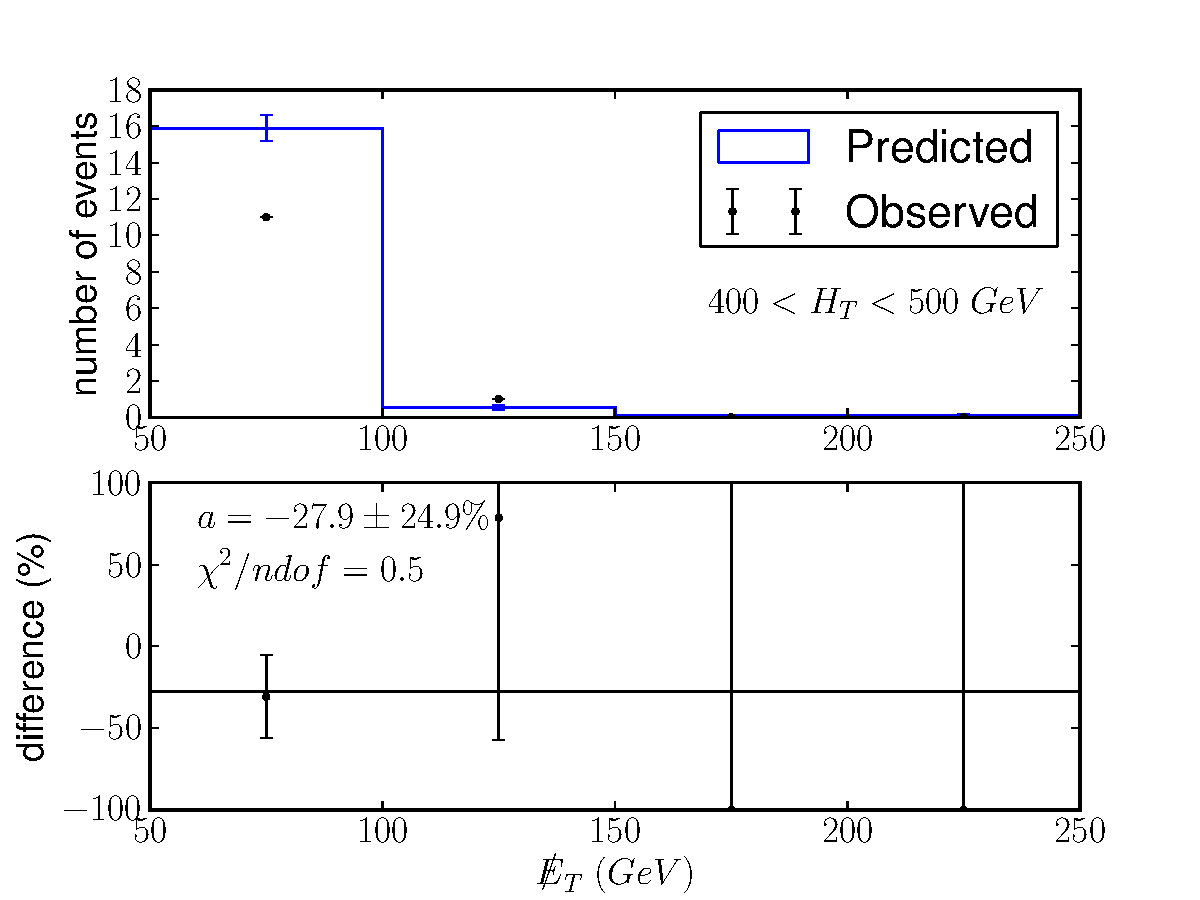
\includegraphics[width=0.5\textwidth]{SB_Bkgd_Est_1.pdf}
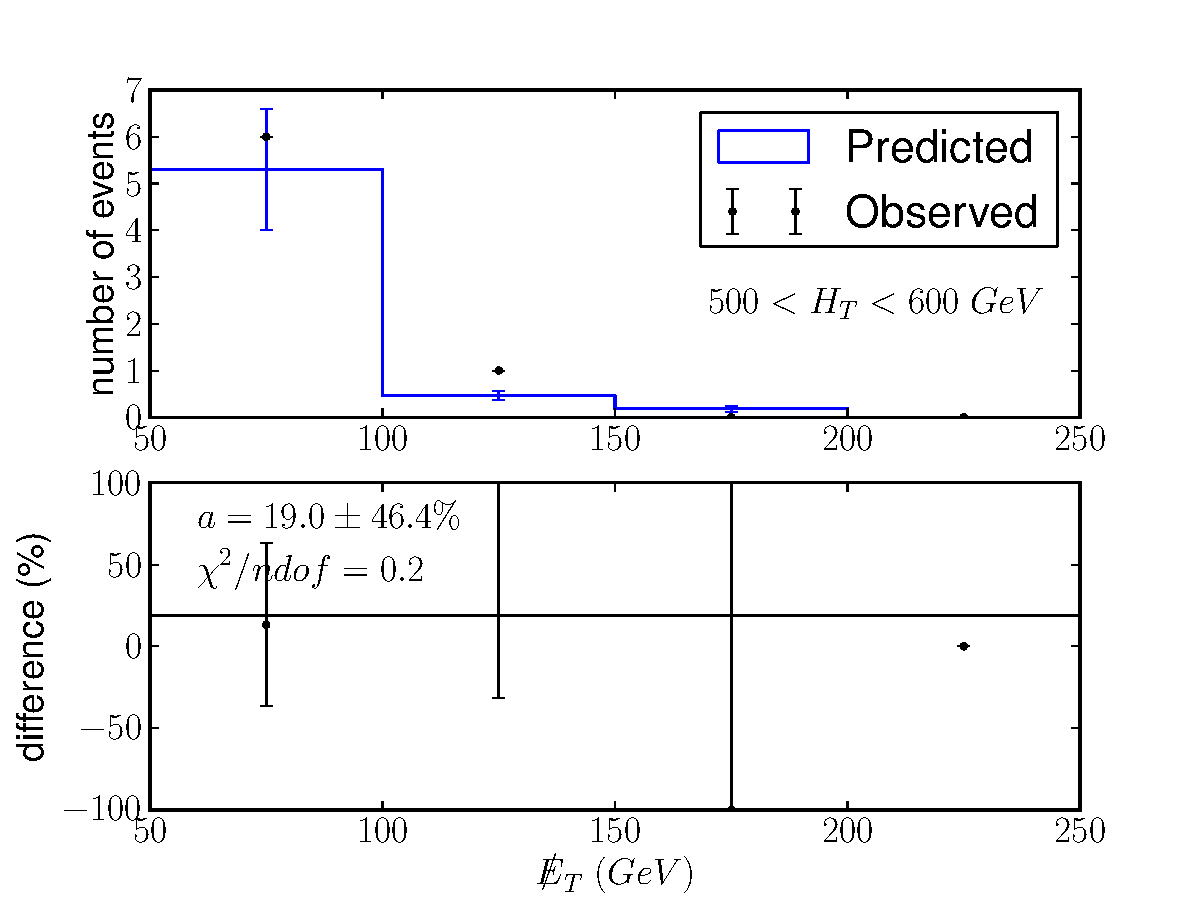
\includegraphics[width=0.5\textwidth]{SB_Bkgd_Est_2.pdf}\\
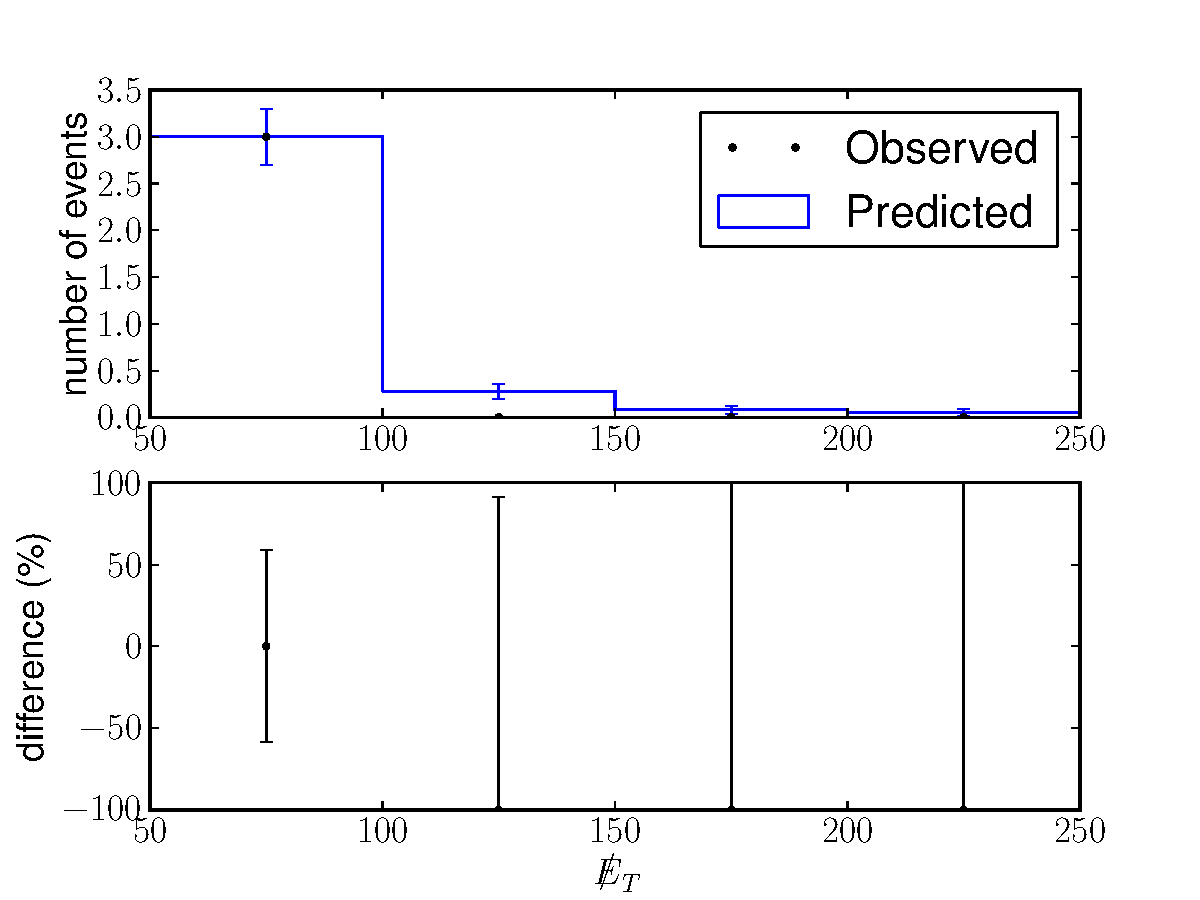
\includegraphics[width=0.5\textwidth]{SB_Bkgd_Est_3.pdf}
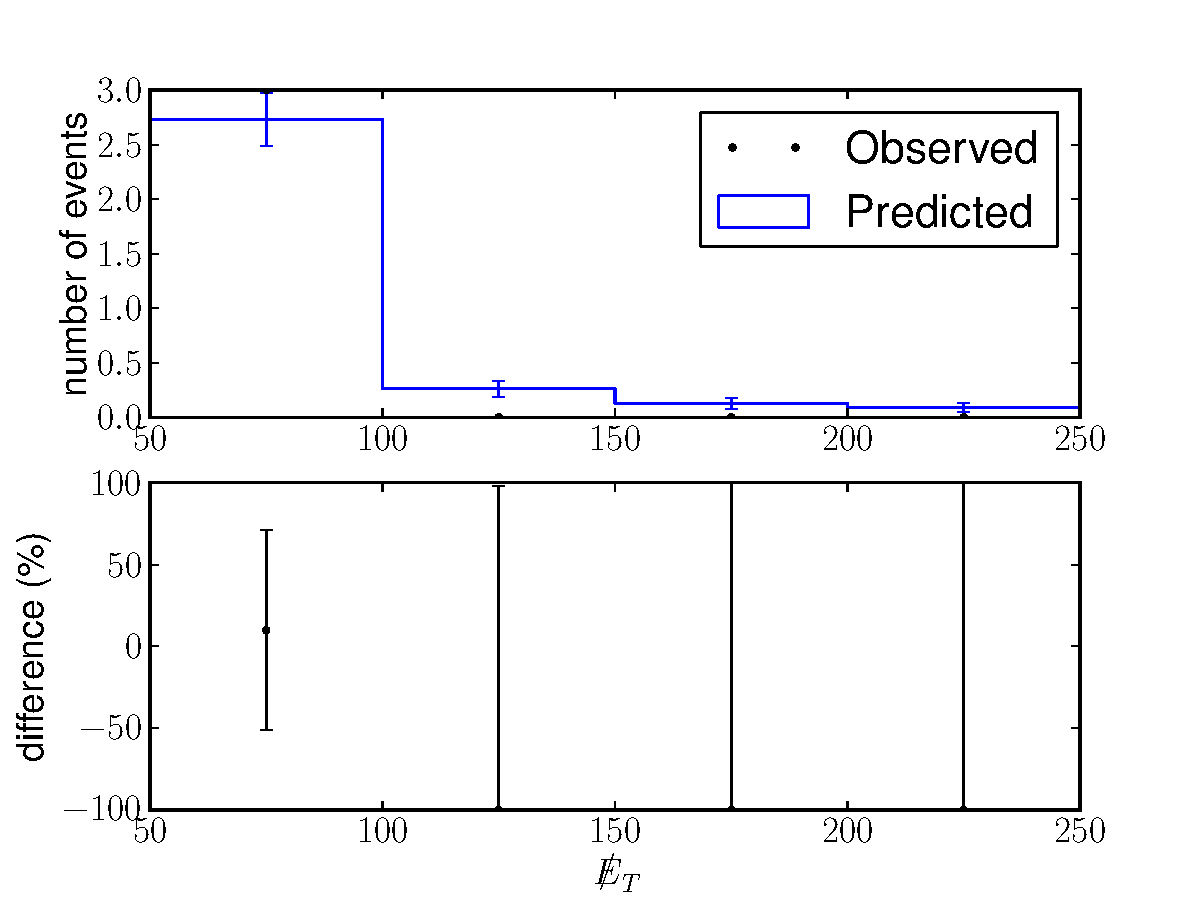
\includegraphics[width=0.5\textwidth]{SB_Bkgd_Est_4.pdf}\\
\caption{The estimated $\MET$ distribution of isolated events using the
non-isolated events in the sideband region compared to the true $\MET$
distribution of the isolated events in the sideband region in bins of $\HT$. The 
percentage difference between the estimated and observed number of events is 
plotted and a flat line is fitted.}
\label{fig:Bkgd_Est_Sideband}
\end{figure}

Now that background estimation procedure has been shown to work using the MC and
using the sideband region, it can be used on the data to make the background
estimation for this search. Figure \ref{fig:Bkgd_Est} shows the $\MET$
distribution of the background estimation in bins of $\HT$. The important number 
for this search is the estimated number of background events in the 
($\HT>700\unit{GeV}$, $\MET>200\unit{GeV}$) bin because that is the most 
significant bin in terms of the limit placed on the GMSB cross-section. The 
estimated number of backgound events in this bin along with its statistical 
uncertainty is $7.7\pm2.1$. \\

\begin{figure}
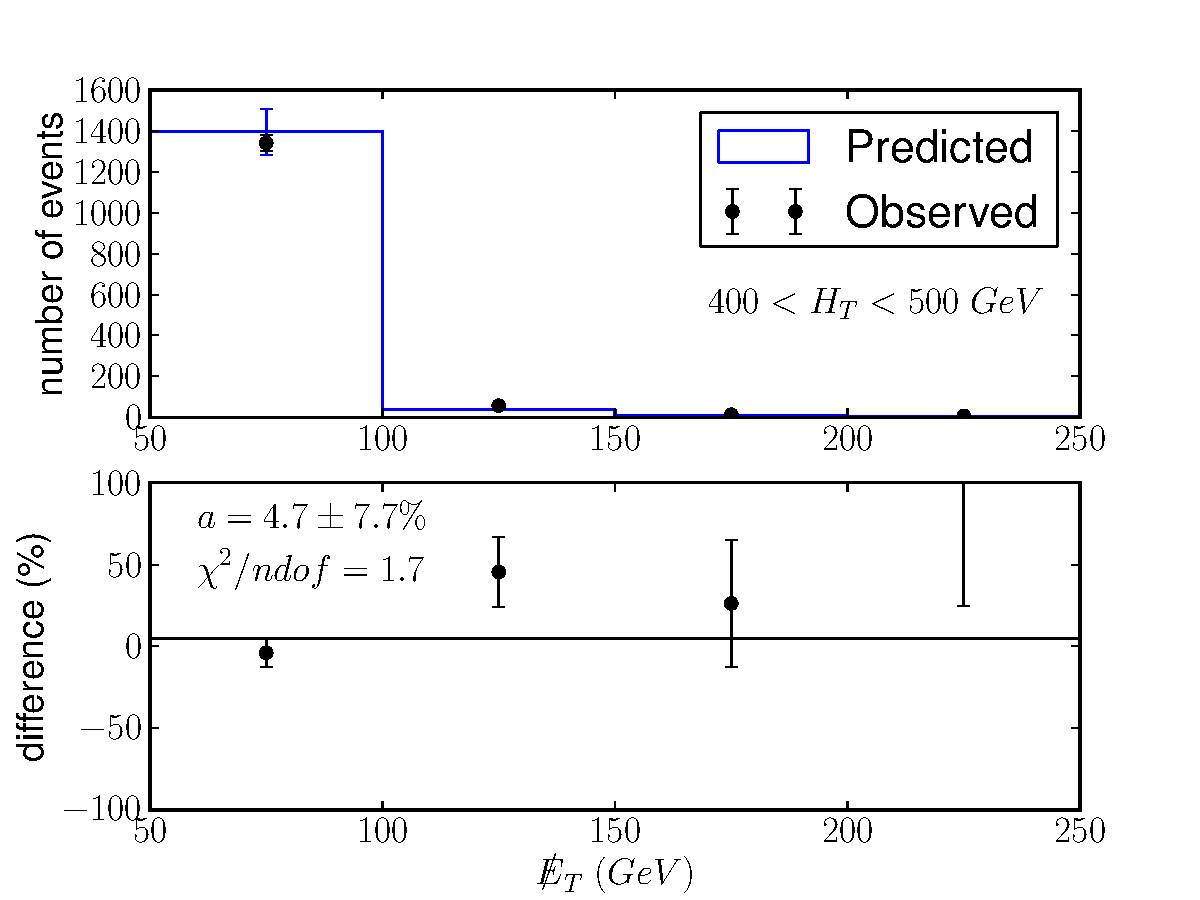
\includegraphics[width=0.5\textwidth]{Bkgd_Est_1.pdf}
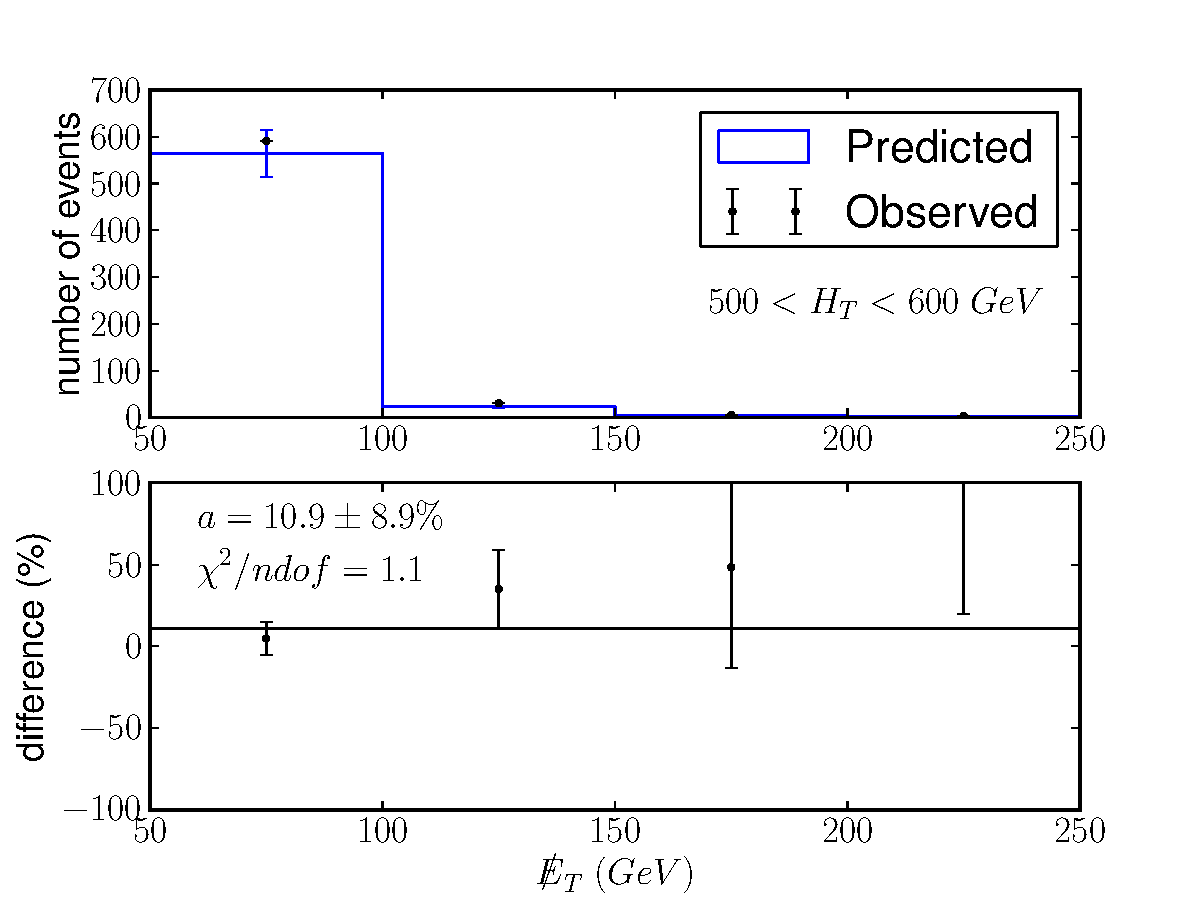
\includegraphics[width=0.5\textwidth]{Bkgd_Est_2.pdf}\\
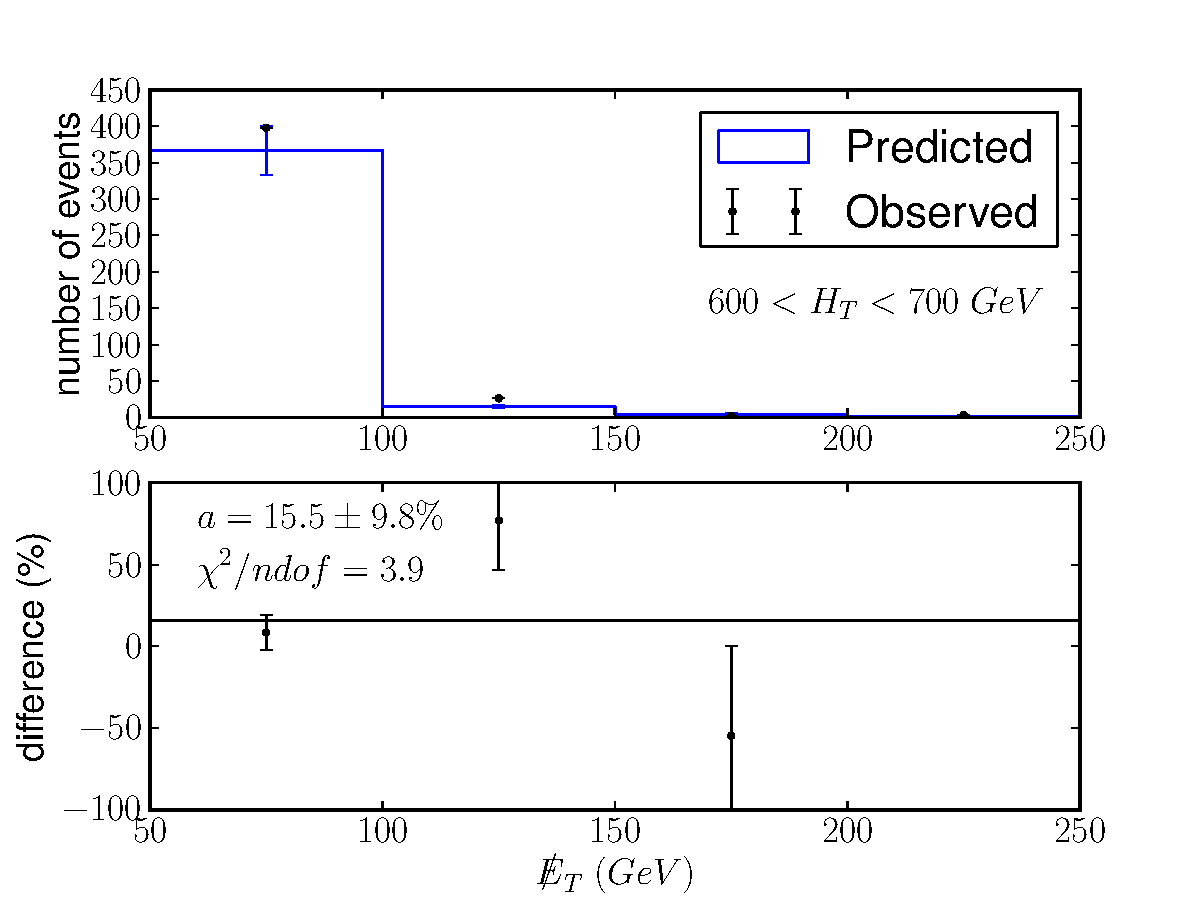
\includegraphics[width=0.5\textwidth]{Bkgd_Est_3.pdf}
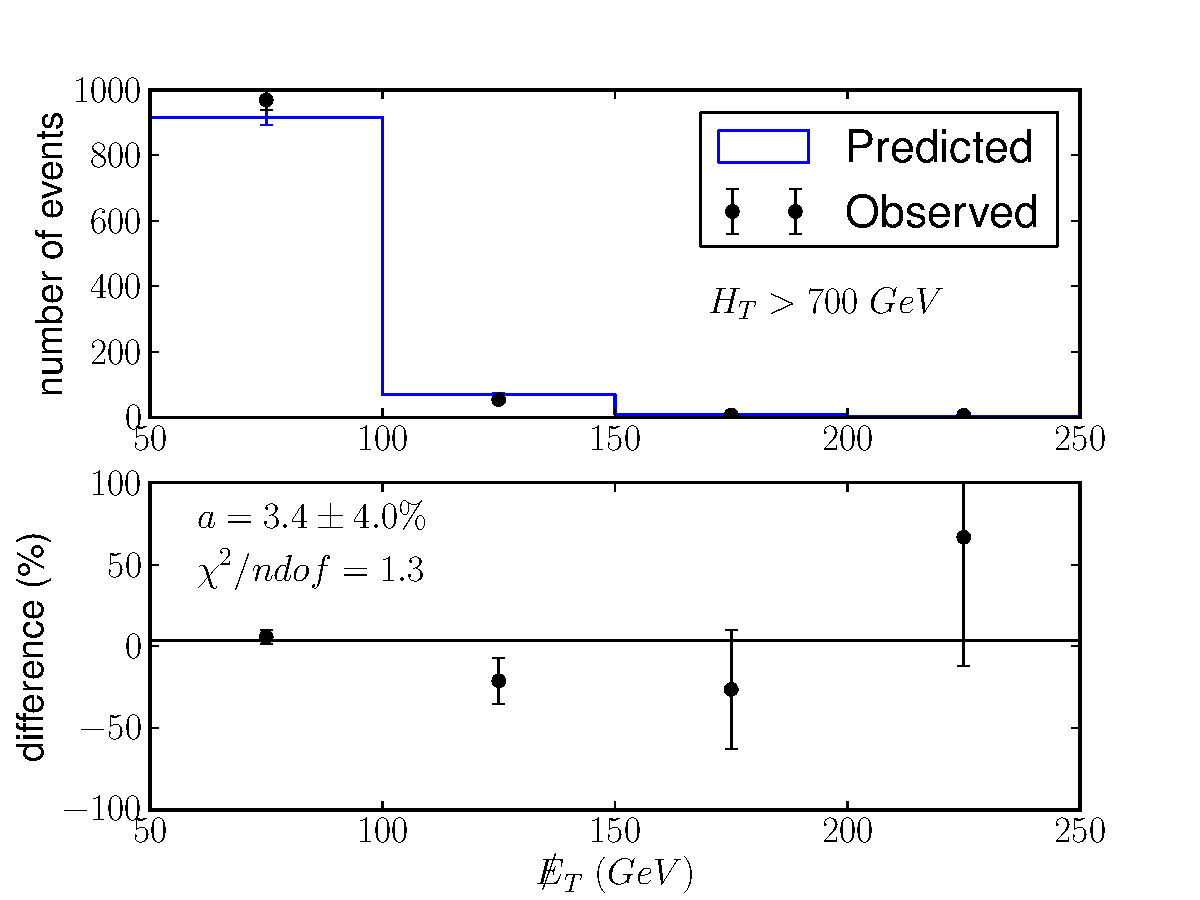
\includegraphics[width=0.5\textwidth]{Bkgd_Est_4.pdf}\\
\caption{The estimated $\MET$ distribution of background using the control
sample compared to the observed $\MET$ distribution of the selected events in 
bins of $\HT$. The percentage difference between the estimated and observed
number of events is plotted and a flat line is fitted.}
\label{fig:Bkgd_Est}
\end{figure}

The systematic uncertainty on the background estimation comes from the assumption 
that the control sample accurately estimates the number of selected events. Due
to the small number of events in the sideband region, the MC alone is used to
determine the systematic uncertainty. The uncertainty has two components: the
uncertainty due to a systematic difference between the estimation and the truth 
in the MC, $\sigma_{\delta}$, and an uncertainty in the values of the estimation 
and the truth due to the statistics of the MC, $\sigma_{stat}$. These two 
components are added in quadrature to get the systematic uncertainty assigned to 
the background estimation (Equation \ref{eq:syst}).

\begin{equation}
\sigma_{total} = \sqrt{\sigma_{\delta}^{2} + \sigma_{stat}^{2}}
\label{eq:syst}
\end{equation}

The value of $\sigma_{\delta}$ is 29\unit{\%} and the value of $\sigma_{stat}$
is 25\unit{\%}. Thus the total systematic uncertainty on the background 
estimation is 38\unit{\%}. The estimate of the number of background events 
including statistical and systematic uncertainties is 
$7.7\pm2.1(stat.)\pm2.7(syst.)$.

\section{Electroweak and $t\bar{t}$ Backgrounds}

The Electroweak background is small in comparison to the QCD background.
Electroweak processes can contribute real $\MET$ through the neutrino which is 
not detected. The cross section of electroweak processes is much lower than
that of QCD and this rules out any background due to fakes from jets. There are
two possible sources of photons: $W\rightarrow e\nu$ where the electron has been
misidentied as a photon or W/Z with ISR/FSR which is negligible due to the high 
$\HT$ requirement. \\

The $W\rightarrow e\nu$ background is estimated using the MC and by measuring 
the electron/photon misidentification rate in data. The misidentification rate 
is measured to be $0.014\pm0.004$ \cite{ra3}. This agrees well with the value 
from MC: $0.012\pm0.002$. The total number of $W\rightarrow e\nu$ events passing 
the selection is $0.52\pm0.10(stat.)$. The W/Z+$\gamma$ background is estimated 
to be $0.030\pm0.030$ from the MC. A conservative estimate of the systematic 
uncertainty of $100\unit{\%}$ is made to cover the jet energy scale, jet energy 
resolution, cross-section and luminosity uncertainties. \\

The $t\bar{t}$ background also has real $\MET$, but it is negligible due to the
low cross-section. The $t\bar{t}$ background is estimated using Monte Carlo to
be $0.007\pm0.007$, where again a systematic uncertainty of $100\unit{\%}$ is
used as conservative estimate. \\

Ignoring the $W/Z+\gamma$ and $t\bar{t}$ backgrounds because they are so small, 
the total electroweak background is $0.5\pm0.5$ events.
 
\section{Conclusions}

The background from QCD processes in the only significant bin
($\HT>700\unit{GeV}$, $\MET>200\unit{GeV}$) is estimated to be 
$7.2\pm2.1(stat.)\pm2.9(syst.)$ events. The background from electroweak
processes is estimated to be $0.5\pm0.5$ events.
